\chapter{Results}

\section*{Preparation}
\begin{figure}[h]
    \centering
    \begin{subfigure}{0.25\textwidth}
        \includegraphics[width = \textwidth]{Plots/Fe.png}
        \caption{}
        \label{fig:leed_Fe}
    \end{subfigure}
    \hfill
    \begin{subfigure}{0.25\textwidth}
        \includegraphics[width = \textwidth]{Plots/FeO.png}
        \caption{}
        \label{fig:leed_FeO}
    \end{subfigure}
    \hfill
    \begin{subfigure}{0.25\textwidth}
        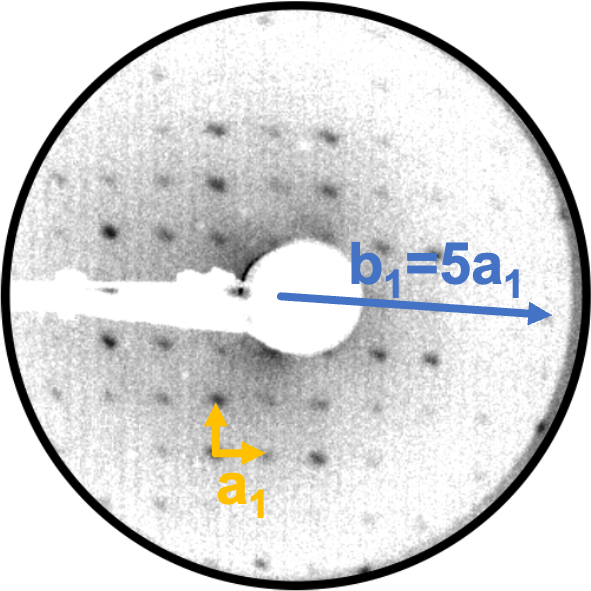
\includegraphics[width = \textwidth]{Plots/FeO_ZnTPP.png}
        \caption{}
        \label{fig:leed_FeO_ZnTPP}
    \end{subfigure}
    \caption{\textbf{(a)} LEED image of the Fe(001) surface at an electron beam energy of \qty{90}{eV}. \textbf{(b)} LEED image of the Fe(001)p-(1\times1)O surface at an electron beam energy of \qty{90}{eV}. \textbf{(c)} LEED image of the Fe(001)p-(1\times1)O/ZnTPP surface at an electron beam energy of \qty{32}{eV}.}
    \label{fig:leed_1}
\end{figure}
\FloatBarrier

To confirm the quality of the Fe monoxide layer a LEED image was taken before and after passivation at the same electron beam energy of \qty{90}{eV}, displayed in Figures \ref{fig:leed_Fe} and \ref{fig:leed_FeO}.
The comparison to the clean surface shows no degradation of the spot sharpness, which indicates a complete monolayer coverage without contamination.
There is also no change in spot position, so that a (1\times1) reconstruction of oxygen atoms can be assumed lying in the grooves between the Fe atoms.
As can be seen in \autoref{fig:leed_FeO_ZnTPP} the ZnTPP forms a commensurate square (5\times5) super-lattice, which shows a certain interaction with the substrate.
The reciprocal lattice constant of the underlying substrate $a_1$ is five times the reciprocal lattice constant of the reconstruction $b_1$, meaning that the ZnTPP molecules are apart $14,25\,$\r{A}, five times the Fe lattice constant $2,85\,$\r{A} [3].

\begin{figure}[h]
    \centering
    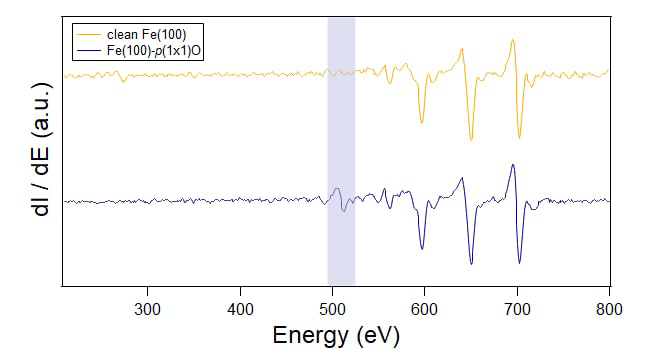
\includegraphics[width = 0.7\textwidth]{Plots/Auger.png}
    \caption{The derivative of the Auger spectrum showing the oxygen peak at \qty{503}{eV}.}
    \label{fig:auger_FeO}
\end{figure}
\FloatBarrier
Comparing the Auger spectra of the clean and passivated Fe surface also shows a significant increase in the peak at \qty{503}{eV} belonging to oxygen.
From a chemical composition point of view this poses as another confirmation, that the Fe surface was passivated.

For the clean Cu substrate a square lattice can be seen in \autoref{fig:leed_Cu}.
After deposition of the ZnTPP molecules on the surface, a complex pattern due to several domains is visible in \autoref{fig:leed_Cu_ZnTPP}.
The corresponding super-lattice is assumed to be incommensurable to the underlying substrate.
\begin{figure}[h]
    \centering
    \begin{subfigure}{0.49\textwidth}
        \centering
        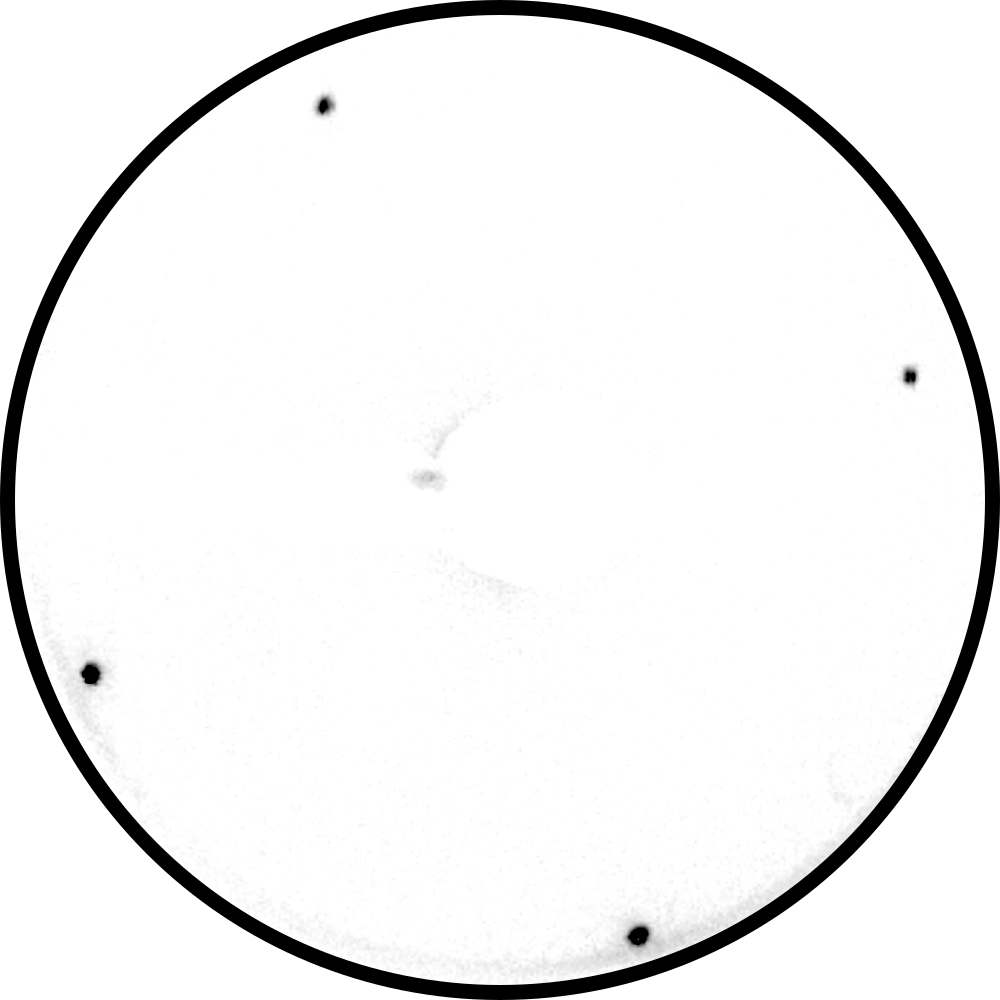
\includegraphics[width = 0.5\textwidth]{Plots/Cu.png}
        \caption{}
        \label{fig:leed_Cu}
    \end{subfigure}
    \hfill
    \begin{subfigure}{0.49\textwidth}
        \centering
        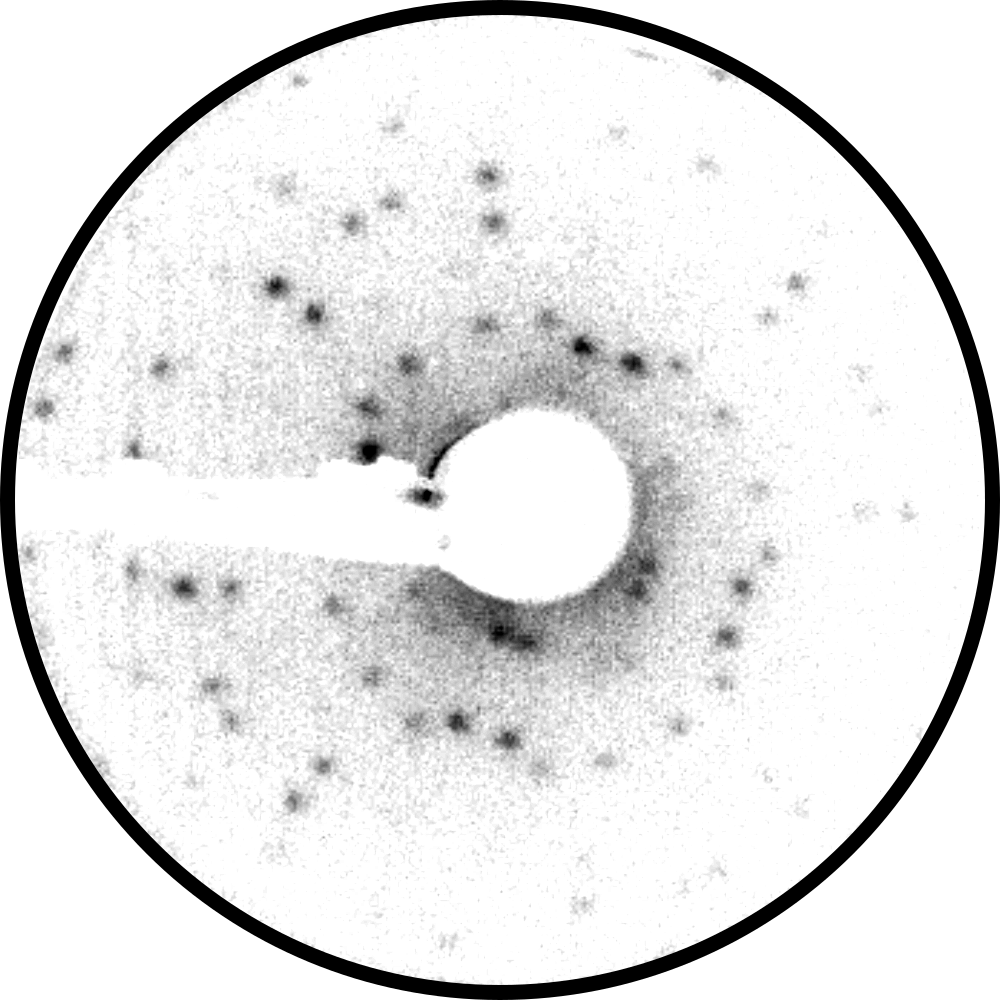
\includegraphics[width = 0.5\textwidth]{Plots/Cu_ZnTPP.png}
        \caption{}
        \label{fig:leed_Cu_ZnTPP}
    \end{subfigure}
    \caption{\textbf{(a)} LEED image of the Cu(100) surface at an electron beam energy of \qty{44}{eV}. \textbf{(b)} LEED image of the Cu(100)/ZnTPP surface at an electron beam energy of \qty{32}{eV}.}
    \label{fig:leed_2}
\end{figure}
\FloatBarrier

\newpage
\section*{Electronic structure characterization}
\begin{figure}[h]
    \centering
    \begin{subfigure}{0.49\textwidth}
        \centering
        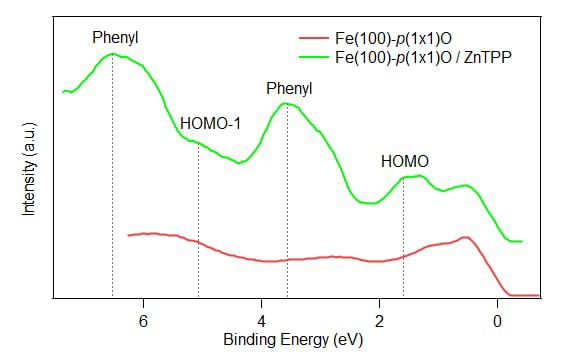
\includegraphics[width = \textwidth]{Plots/integrated_spectrum_Fe.png}
        \caption{}
        \label{fig:ups_spectrum}
    \end{subfigure}
    \hfill
    \begin{subfigure}{0.49\textwidth}
        \centering
        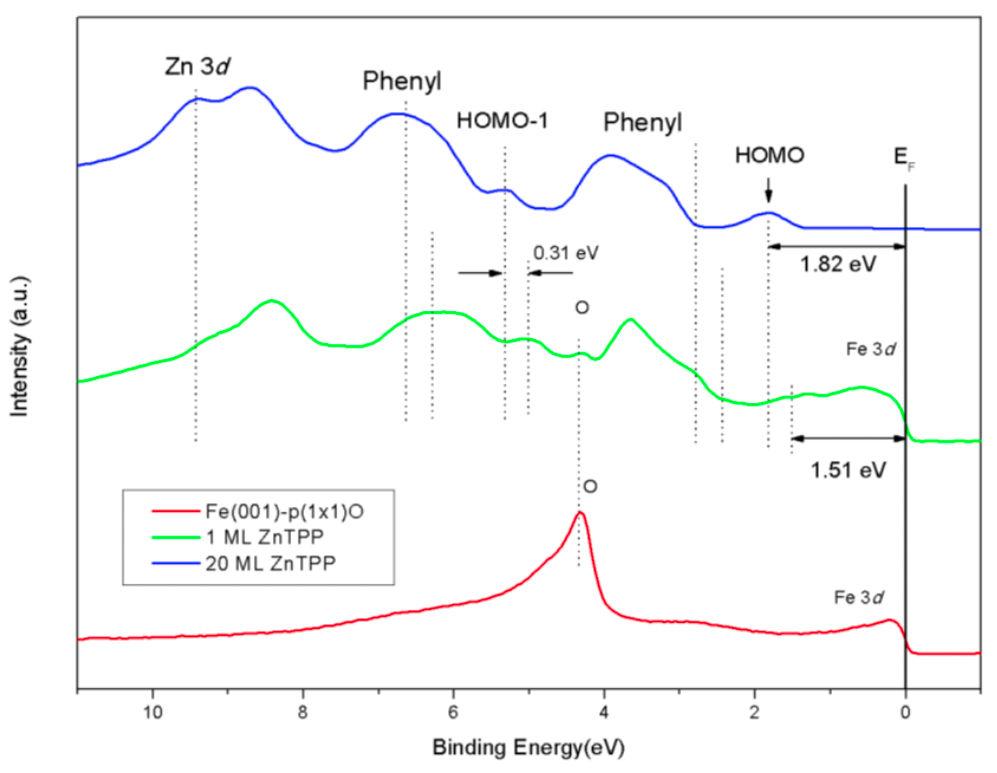
\includegraphics[width = \textwidth]{Plots/integrated_spectrum_Fe_lit.png}
        \caption{}
        \label{fig:ups_spectrum_lit}
    \end{subfigure}
    \caption{\textbf{(a)} The UPS spectrum measured for the Fe(001)p-(1\times1)O substrate and adsorbed ZnTPP monolayer at a photon energy of $h\nu = \qty{29.8}{eV}$. \textbf{(b)} The UPS spectrum for the Fe(001)p-(1\times1)O system taken from [...].}
    \label{fig:ups}
\end{figure}
\FloatBarrier
Using the UPS spectrum \autoref{fig:ups_spectrum_lit} taken from literature [...] the main features of our measured spectrum in \autoref{fig:ups_spectrum} could be identified.
For the red line in \autoref{fig:ups} denoting the UPS spectrum of the clean Fe(001)p-(1\times1)O surface, no oxygen related peak can be discerned, although the bandstructure in \autoref{fig:bandstructure}c) shows a feature in the range of \qty{4.2}{eV}.
The green line corresponds to the Fe(001)p-(1\times1)O/ZnTPP system and here the main electronic peaks can be matched to the ones from the literature.
The HOMO is measured to be at \qty{1.6}{eV} and the HOMO-1 at approximately \qty{5.1}{eV}, which coincides well with the values in \autoref{fig:ups_spectrum_lit}.

The UPS spectrum of Cu/ZnTPP showing no significant changes, is not presented here, as no relevant information can be gained from it.
Because the wide UPS spectra was measured last, after the workfunction, which showed a great difference and based on this outcome it is plausible to say that the ZnTPP molecules somehow desorbed from the surface.

\begin{figure}[h]
    \centering
    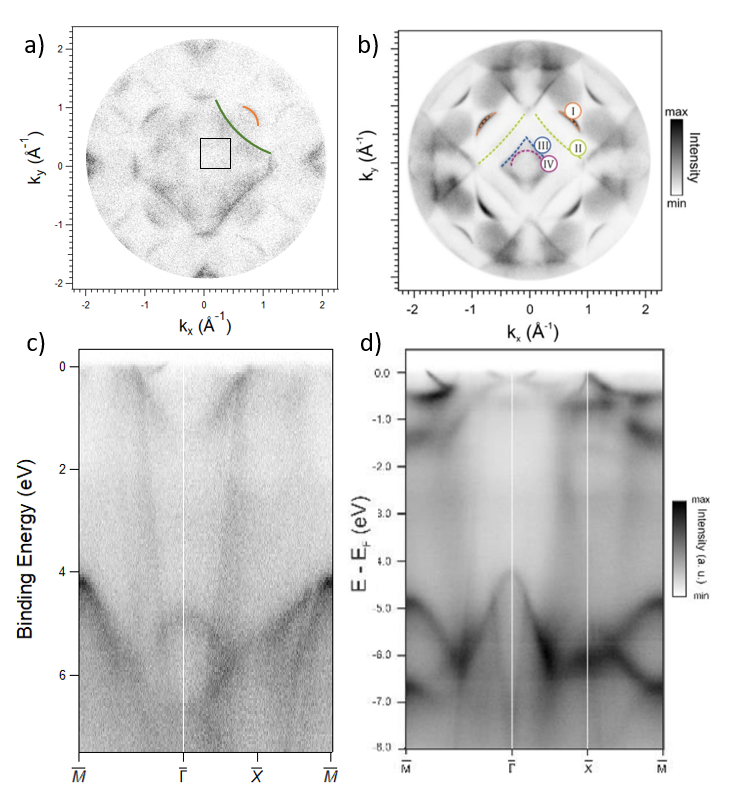
\includegraphics[width = 0.7\textwidth]{Plots/bandstructure.png}
    \caption{\textbf{(a)} .}
    \label{fig:bandstructure}
\end{figure}
\FloatBarrier

Now the work functions for the two samples with and without ZnTPP coverage are calculated by extrapolating the onset intersection with the energy axis. Only the difference between the work functions is important for us, because the origin of the energy axis is set by the chosen sample bias voltage.
In both cases the work function gets reduced.
For the Fe substrate there is a shift of $\Delta\Phi = \qty{0.31}{eV}$ and 
\begin{figure}[h]
    \centering
    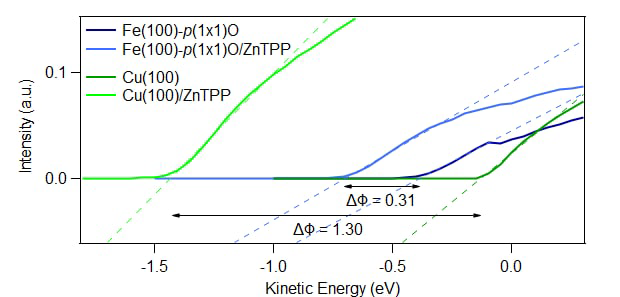
\includegraphics[width = 0.7\textwidth]{Plots/WF.png}
    \caption{Depicting the calculation of the workfunction on the UPS spectra for the Fe and Cu substrate and ZnTPP monolayers.}
    \label{fig:wf}
\end{figure}
\FloatBarrier
